% Ledger diagrams of three approaches in the literature read for Paper A1,
% 17 October 2026. One page per approach.
%   pdflatex -output-directory=build notes/ledger_literature.tex
% The decisions behind each drawing are in notes/ledger_literature.md. Labels
% cite the source's equations, figures and propositions and the quotation IDs
% of its record under lit/. The Lean theorem behind each solid arrow is named
% in the note.
\documentclass[tikz,border=10pt]{standalone}
\usepackage[T1]{fontenc}
\usepackage{helvet}
\renewcommand{\familydefault}{\sfdefault}
\usepackage{amsmath}
\usetikzlibrary{arrows.meta,positioning,fit,calc,backgrounds}
\tikzset{
  >={Stealth[length=2.2mm]},
  every node/.style={font=\small},
  role/.style={draw=black!60, line width=0.5pt, align=center, text width=4.0cm, minimum height=4.2cm, inner sep=4pt, rounded corners=4pt, fill=blue!10},
  pop/.style={draw=black!60, line width=0.5pt, align=center, text width=4.6cm, minimum height=1.2cm, inner sep=4pt, fill=black!8},
  other/.style={draw=black!60, line width=0.7pt, align=center, text width=4.8cm, minimum height=4.2cm, inner sep=5pt, rounded corners=4pt, fill=orange!15},
  entity/.style={draw=black!80, line width=0.8pt, rounded corners=8pt, inner sep=10pt, fill=blue!3},
  etitle/.style={font=\small\bfseries, anchor=north west, align=left},
  attr/.style={font=\scriptsize, anchor=north west, align=left, text width=6.2cm},
  lab/.style={font=\scriptsize, align=center, fill=white, inner sep=1.2pt, text width=3.0cm},
  note/.style={draw=black!40, dashed, font=\scriptsize, align=left, text width=9.5cm, inner sep=5pt, fill=yellow!8},
  head/.style={font=\small, align=left, anchor=south west, text width=26cm},
  settled/.style={->, line width=0.6pt},
  given/.style={->, line width=0.6pt, dashed},
  open/.style={->, line width=0.6pt, dotted, line cap=round},
  jointgiven/.style={<->, line width=0.6pt, dashed},
}
\newcommand{\legend}{Solid = derived in the paper and proved in the Lean record. \quad Dashed = assumed by the paper, or claimed by it and not formalised in the record. \quad Dotted = stated in words, not modelled. \quad ``Recorded as'' marks what the data record.}

\begin{document}

% =====================================================================
% 1. Statistical discrimination, Phelps (1972) and Aigner and Cain (1977)
% =====================================================================
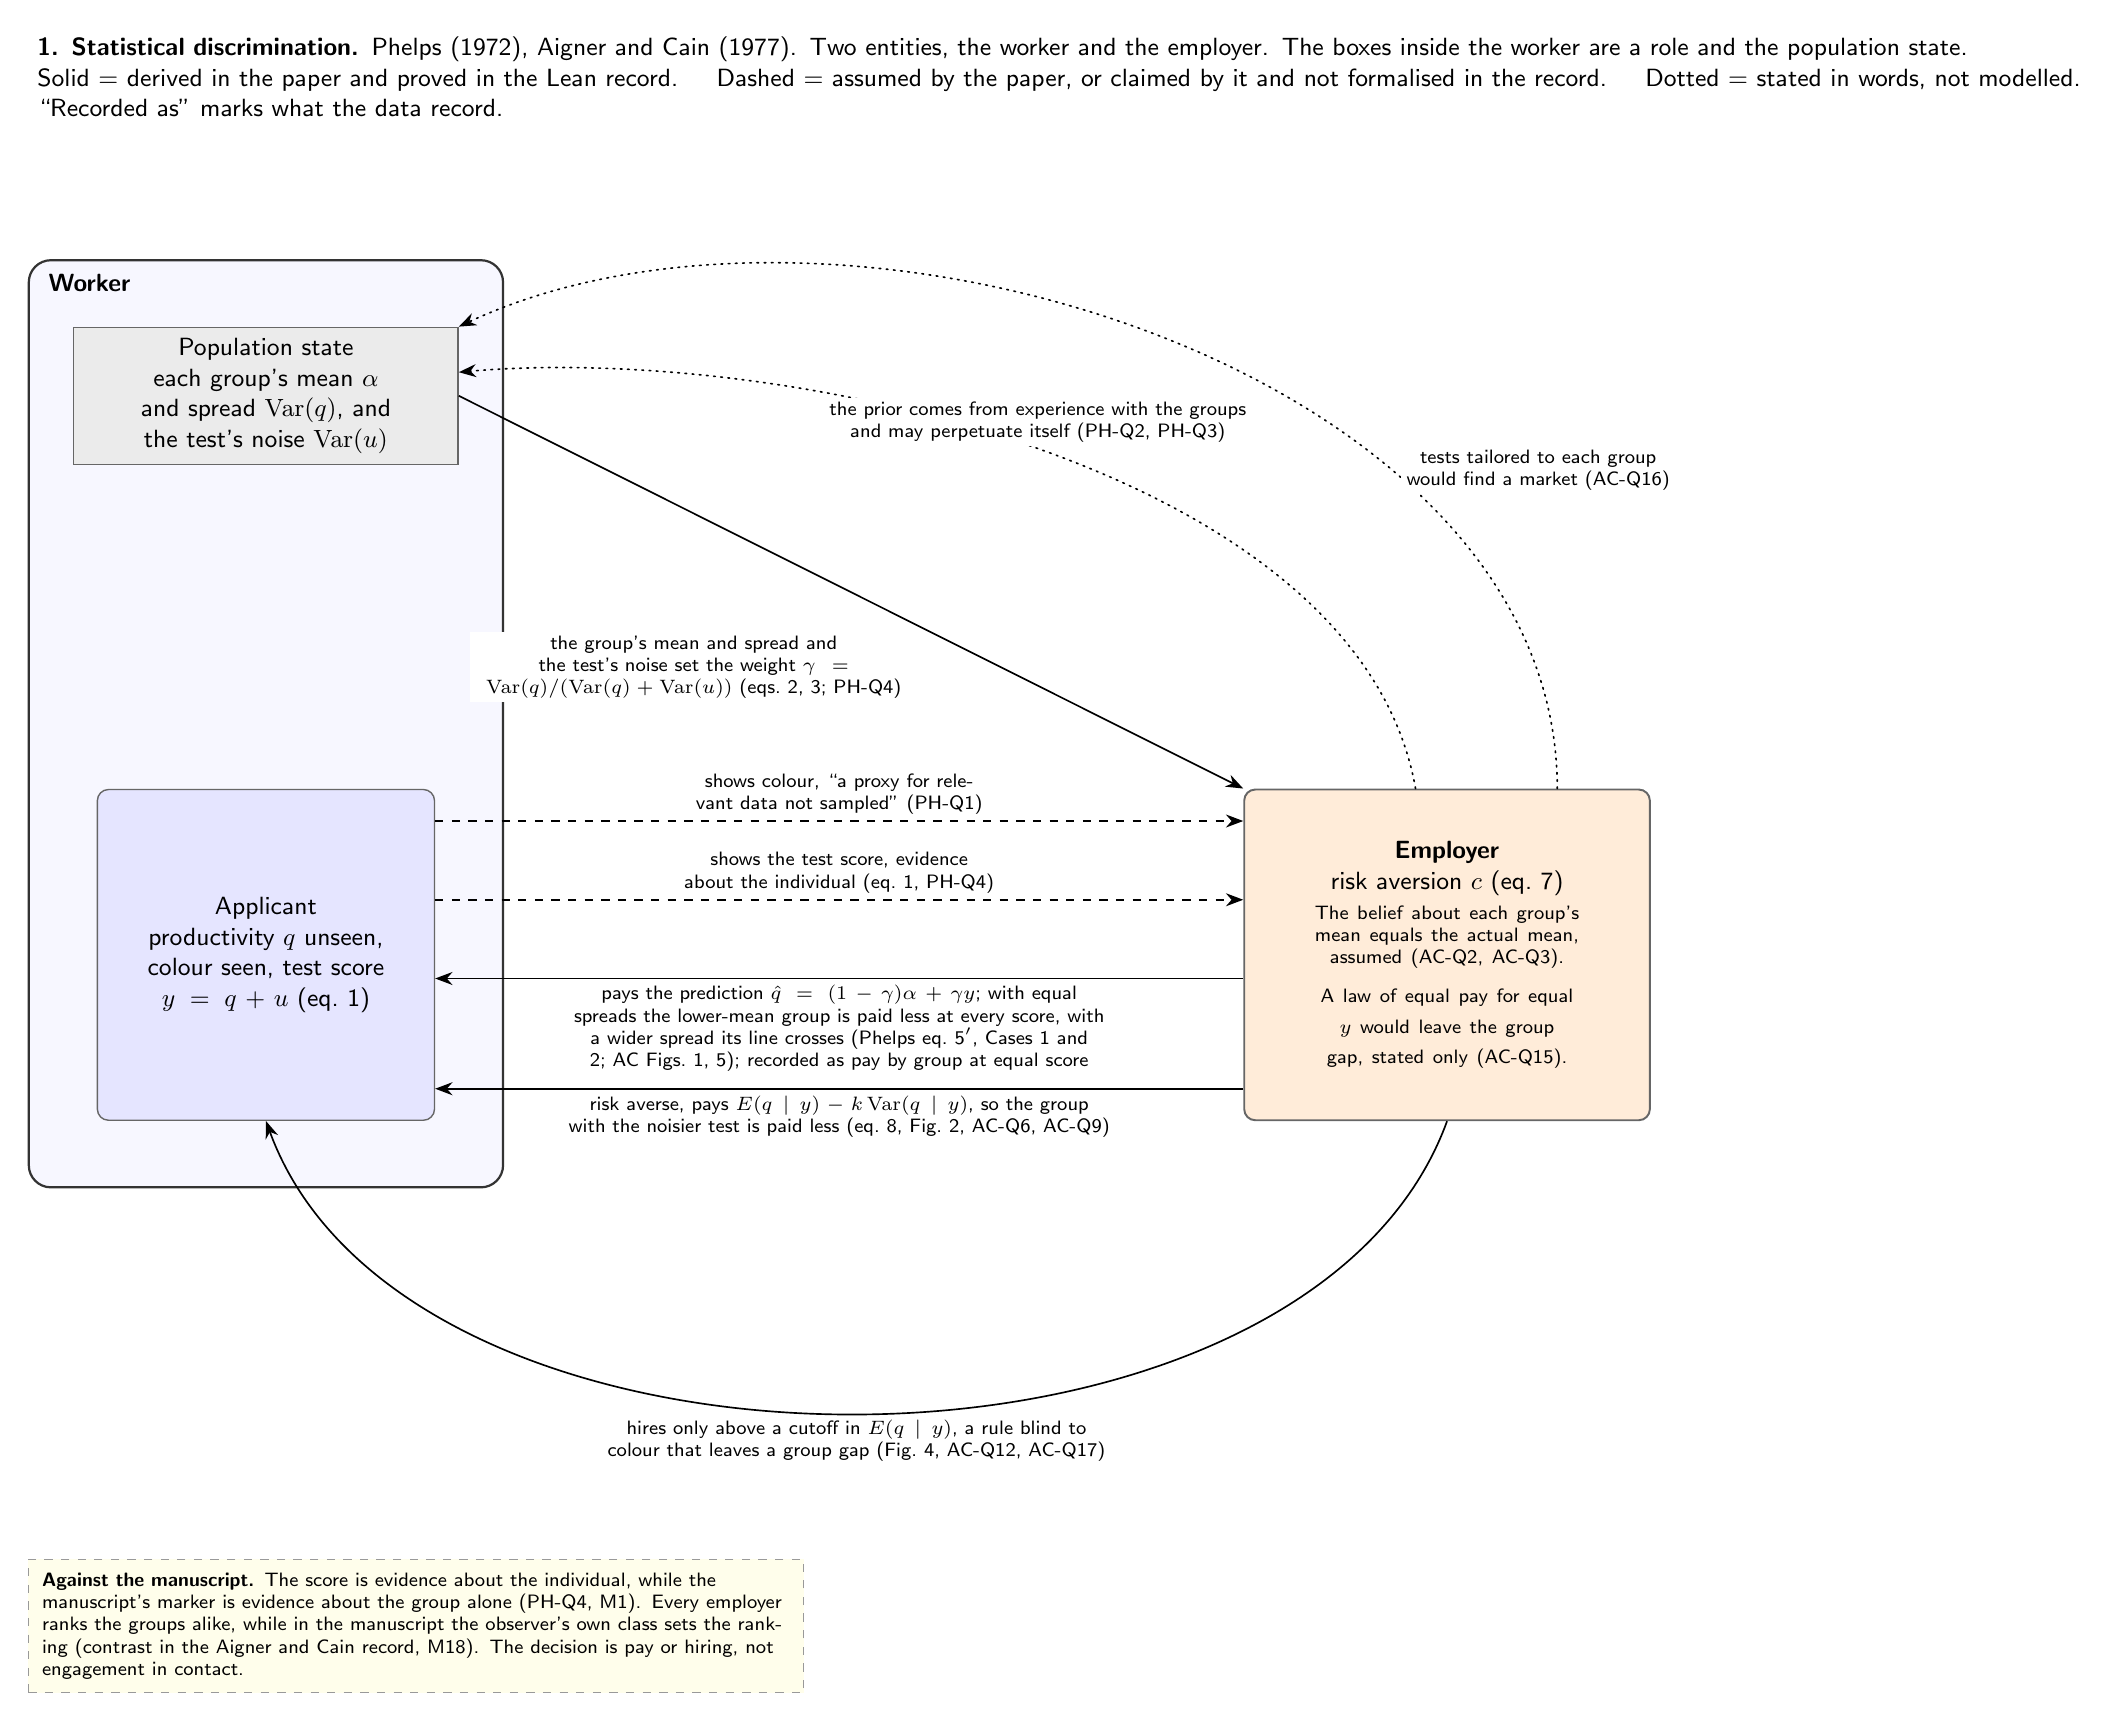
\begin{tikzpicture}
\node[pop]  (Pop) at (4,8.6) {Population state\\ each group's mean $\alpha$ and spread $\mathrm{Var}(q)$, and the test's noise $\mathrm{Var}(u)$};
\node[role] (App) at (4,1.5) {Applicant\\ productivity $q$ unseen, colour seen, test score $y=q+u$ (eq.~1)};
\begin{scope}[on background layer]
\node[entity, fit=(Pop)(App), inner xsep=16pt, inner ysep=24pt] (WBox) {};
\end{scope}
\node[etitle] at ([xshift=4pt, yshift=-2pt]WBox.north west) {Worker};

\node[other] (Emp) at (19,1.5) {\textbf{Employer}\\ risk aversion $c$ (eq.~7)\\[3pt] \scriptsize The belief about each group's mean equals the actual mean, assumed (AC-Q2, AC-Q3).\\[3pt] \scriptsize A law of equal pay for equal $y$ would leave the group gap, stated only (AC-Q15).};

\draw[given]   ([yshift=17mm]App.east) -- node[lab, pos=0.5, above=1pt, text width=6cm] {shows colour, ``a proxy for relevant data not sampled'' (PH-Q1)} ([yshift=17mm]Emp.west);
\draw[given]   ([yshift=7mm]App.east) -- node[lab, pos=0.5, above=1pt, text width=6cm] {shows the test score, evidence about the individual (eq.~1, PH-Q4)} ([yshift=7mm]Emp.west);
\draw[settled] ([yshift=-3mm]Emp.west) -- node[lab, pos=0.5, below=1pt, text width=7.4cm] {pays the prediction $\hat q=(1-\gamma)\alpha+\gamma y$; with equal spreads the lower-mean group is paid less at every score, with a wider spread its line crosses (Phelps eq.~5$'$, Cases 1 and 2; AC Figs.~1, 5); recorded as pay by group at equal score} ([yshift=-3mm]App.east);
\draw[settled] ([yshift=-17mm]Emp.west) -- node[lab, pos=0.5, below=1pt, text width=7.0cm] {risk averse, pays $E(q\mid y)-k\,\mathrm{Var}(q\mid y)$, so the group with the noisier test is paid less (eq.~8, Fig.~2, AC-Q6, AC-Q9)} ([yshift=-17mm]App.east);
\draw[settled] (Emp.south) to[out=-110, in=-70, looseness=0.9] node[lab, pos=0.5, below=1pt, text width=6.5cm] {hires only above a cutoff in $E(q\mid y)$, a rule blind to colour that leaves a group gap (Fig.~4, AC-Q12, AC-Q17)} (App.south);
\draw[settled] (Pop.east) -- node[lab, pos=0.6, anchor=north east, xshift=-4pt, text width=5.6cm] {the group's mean and spread and the test's noise set the weight $\gamma=\mathrm{Var}(q)/(\mathrm{Var}(q)+\mathrm{Var}(u))$ (eqs.~2, 3; PH-Q4)} (Emp.north west);
\draw[open]    ([xshift=-4mm]Emp.north) to[out=100, in=5, looseness=0.8] node[lab, pos=0.5, above=1pt, text width=5.4cm] {the prior comes from experience with the groups and may perpetuate itself (PH-Q2, PH-Q3)} ([yshift=3mm]Pop.east);
\draw[open]    ([xshift=14mm]Emp.north) to[out=90, in=25, looseness=0.9] node[lab, pos=0.3, anchor=west, xshift=3pt, text width=3.4cm] {tests tailored to each group would find a market (AC-Q16)} (Pop.north east);

\node[note, anchor=north west] at ([yshift=-6mm]current bounding box.south west) {\textbf{Against the manuscript.} The score is evidence about the individual, while the manuscript's marker is evidence about the group alone (PH-Q4, M1). Every employer ranks the groups alike, while in the manuscript the observer's own class sets the ranking (contrast in the Aigner and Cain record, M18). The decision is pay or hiring, not engagement in contact.};
\node[head] at ([yshift=8pt]current bounding box.north west) {\textbf{1. Statistical discrimination.} Phelps (1972), Aigner and Cain (1977). Two entities, the worker and the employer. The boxes inside the worker are a role and the population state.\\ \legend};
\end{tikzpicture}

% =====================================================================
% 2. Categorisation, Fryer and Jackson (2008)
% =====================================================================
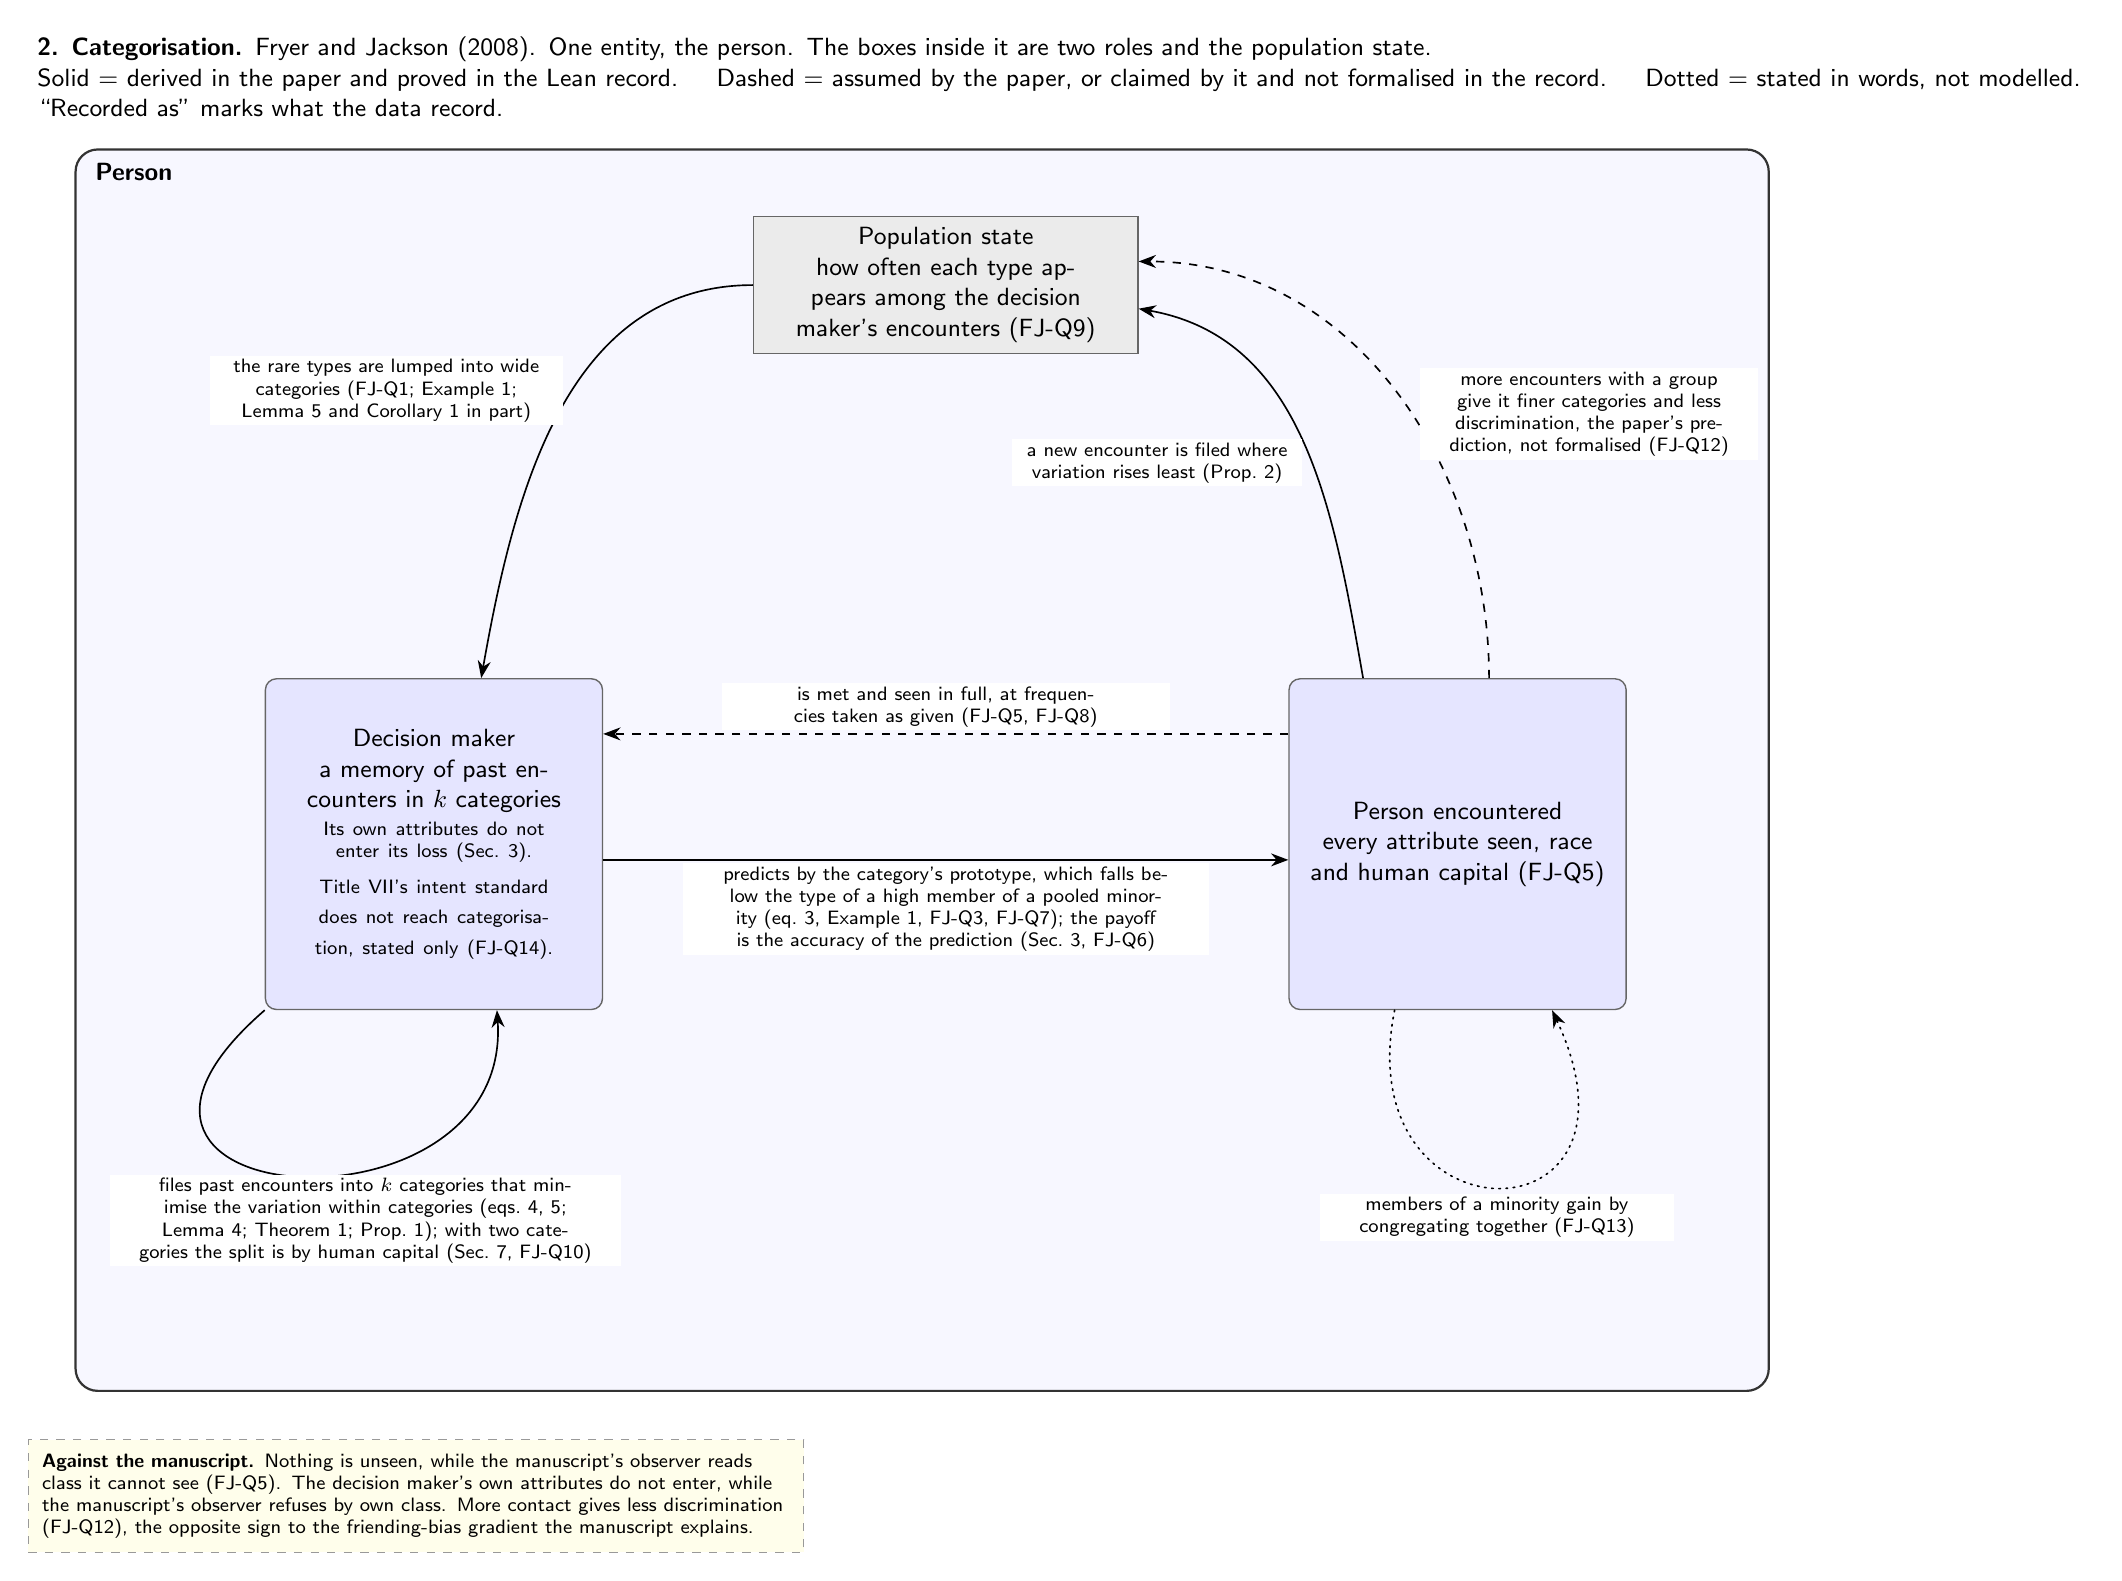
\begin{tikzpicture}
\node[pop]  (Pop) at (6.5,8.6) {Population state\\ how often each type appears among the decision maker's encounters (FJ-Q9)};
\node[role] (DM)  at (0,1.5)   {Decision maker\\ a memory of past encounters in $k$ categories\\[2pt] \scriptsize Its own attributes do not enter its loss (Sec.~3).\\[2pt] \scriptsize Title VII's intent standard does not reach categorisation, stated only (FJ-Q14).};
\node[role] (PE)  at (13,1.5)  {Person encountered\\ every attribute seen, race and human capital (FJ-Q5)};
\begin{scope}[on background layer]
\coordinate (lowL) at (-4.2,-4.6);
\coordinate (lowR) at (16.6,-4.6);
\node[entity, fit=(Pop)(DM)(PE)(lowL)(lowR), inner xsep=10pt, inner ysep=24pt] (PBox) {};
\end{scope}
\node[etitle] at ([xshift=4pt, yshift=-2pt]PBox.north west) {Person};

\draw[given]   ([yshift=14mm]PE.west) -- node[lab, pos=0.5, above=1pt, text width=5.6cm] {is met and seen in full, at frequencies taken as given (FJ-Q5, FJ-Q8)} ([yshift=14mm]DM.east);
\draw[settled] ([yshift=-2mm]DM.east) -- node[lab, pos=0.5, below=1pt, text width=6.6cm] {predicts by the category's prototype, which falls below the type of a high member of a pooled minority (eq.~3, Example~1, FJ-Q3, FJ-Q7); the payoff is the accuracy of the prediction (Sec.~3, FJ-Q6)} ([yshift=-2mm]PE.west);
\draw[settled] (DM.south west) .. controls ([xshift=-30mm, yshift=-26mm]DM.south west) and ([xshift=10mm, yshift=-30mm]DM.south) .. node[lab, pos=0.62, below=2pt, text width=6.4cm] {files past encounters into $k$ categories that minimise the variation within categories (eqs.~4, 5; Lemma~4; Theorem~1; Prop.~1); with two categories the split is by human capital (Sec.~7, FJ-Q10)} ([xshift=8mm]DM.south);
\draw[settled] (Pop.west) to[out=180, in=80] node[lab, pos=0.45, anchor=east, xshift=-3pt, text width=4.4cm] {the rare types are lumped into wide categories (FJ-Q1; Example~1; Lemma~5 and Corollary~1 in part)} ([xshift=6mm]DM.north);
\draw[settled] ([xshift=-12mm]PE.north) to[out=100, in=-10] node[lab, pos=0.45, anchor=east, xshift=-3pt, text width=3.6cm] {a new encounter is filed where variation rises least (Prop.~2)} ([yshift=-3mm]Pop.east);
\draw[given]   ([xshift=4mm]PE.north) to[out=90, in=0] node[lab, pos=0.45, anchor=west, xshift=3pt, text width=4.2cm] {more encounters with a group give it finer categories and less discrimination, the paper's prediction, not formalised (FJ-Q12)} ([yshift=3mm]Pop.east);
\draw[open]    ([xshift=-8mm]PE.south) .. controls ([xshift=-14mm, yshift=-30mm]PE.south) and ([xshift=26mm, yshift=-30mm]PE.south) .. node[lab, pos=0.5, below=2pt, text width=4.4cm] {members of a minority gain by congregating together (FJ-Q13)} ([xshift=12mm]PE.south);

\node[note, anchor=north west] at ([yshift=-6mm]current bounding box.south west) {\textbf{Against the manuscript.} Nothing is unseen, while the manuscript's observer reads class it cannot see (FJ-Q5). The decision maker's own attributes do not enter, while the manuscript's observer refuses by own class. More contact gives less discrimination (FJ-Q12), the opposite sign to the friending-bias gradient the manuscript explains.};
\node[head] at ([yshift=8pt]current bounding box.north west) {\textbf{2. Categorisation.} Fryer and Jackson (2008). One entity, the person. The boxes inside it are two roles and the population state.\\ \legend};
\end{tikzpicture}

% =====================================================================
% 3. Choice and chance in friendship, Currarini, Jackson and Pin (2008)
% =====================================================================
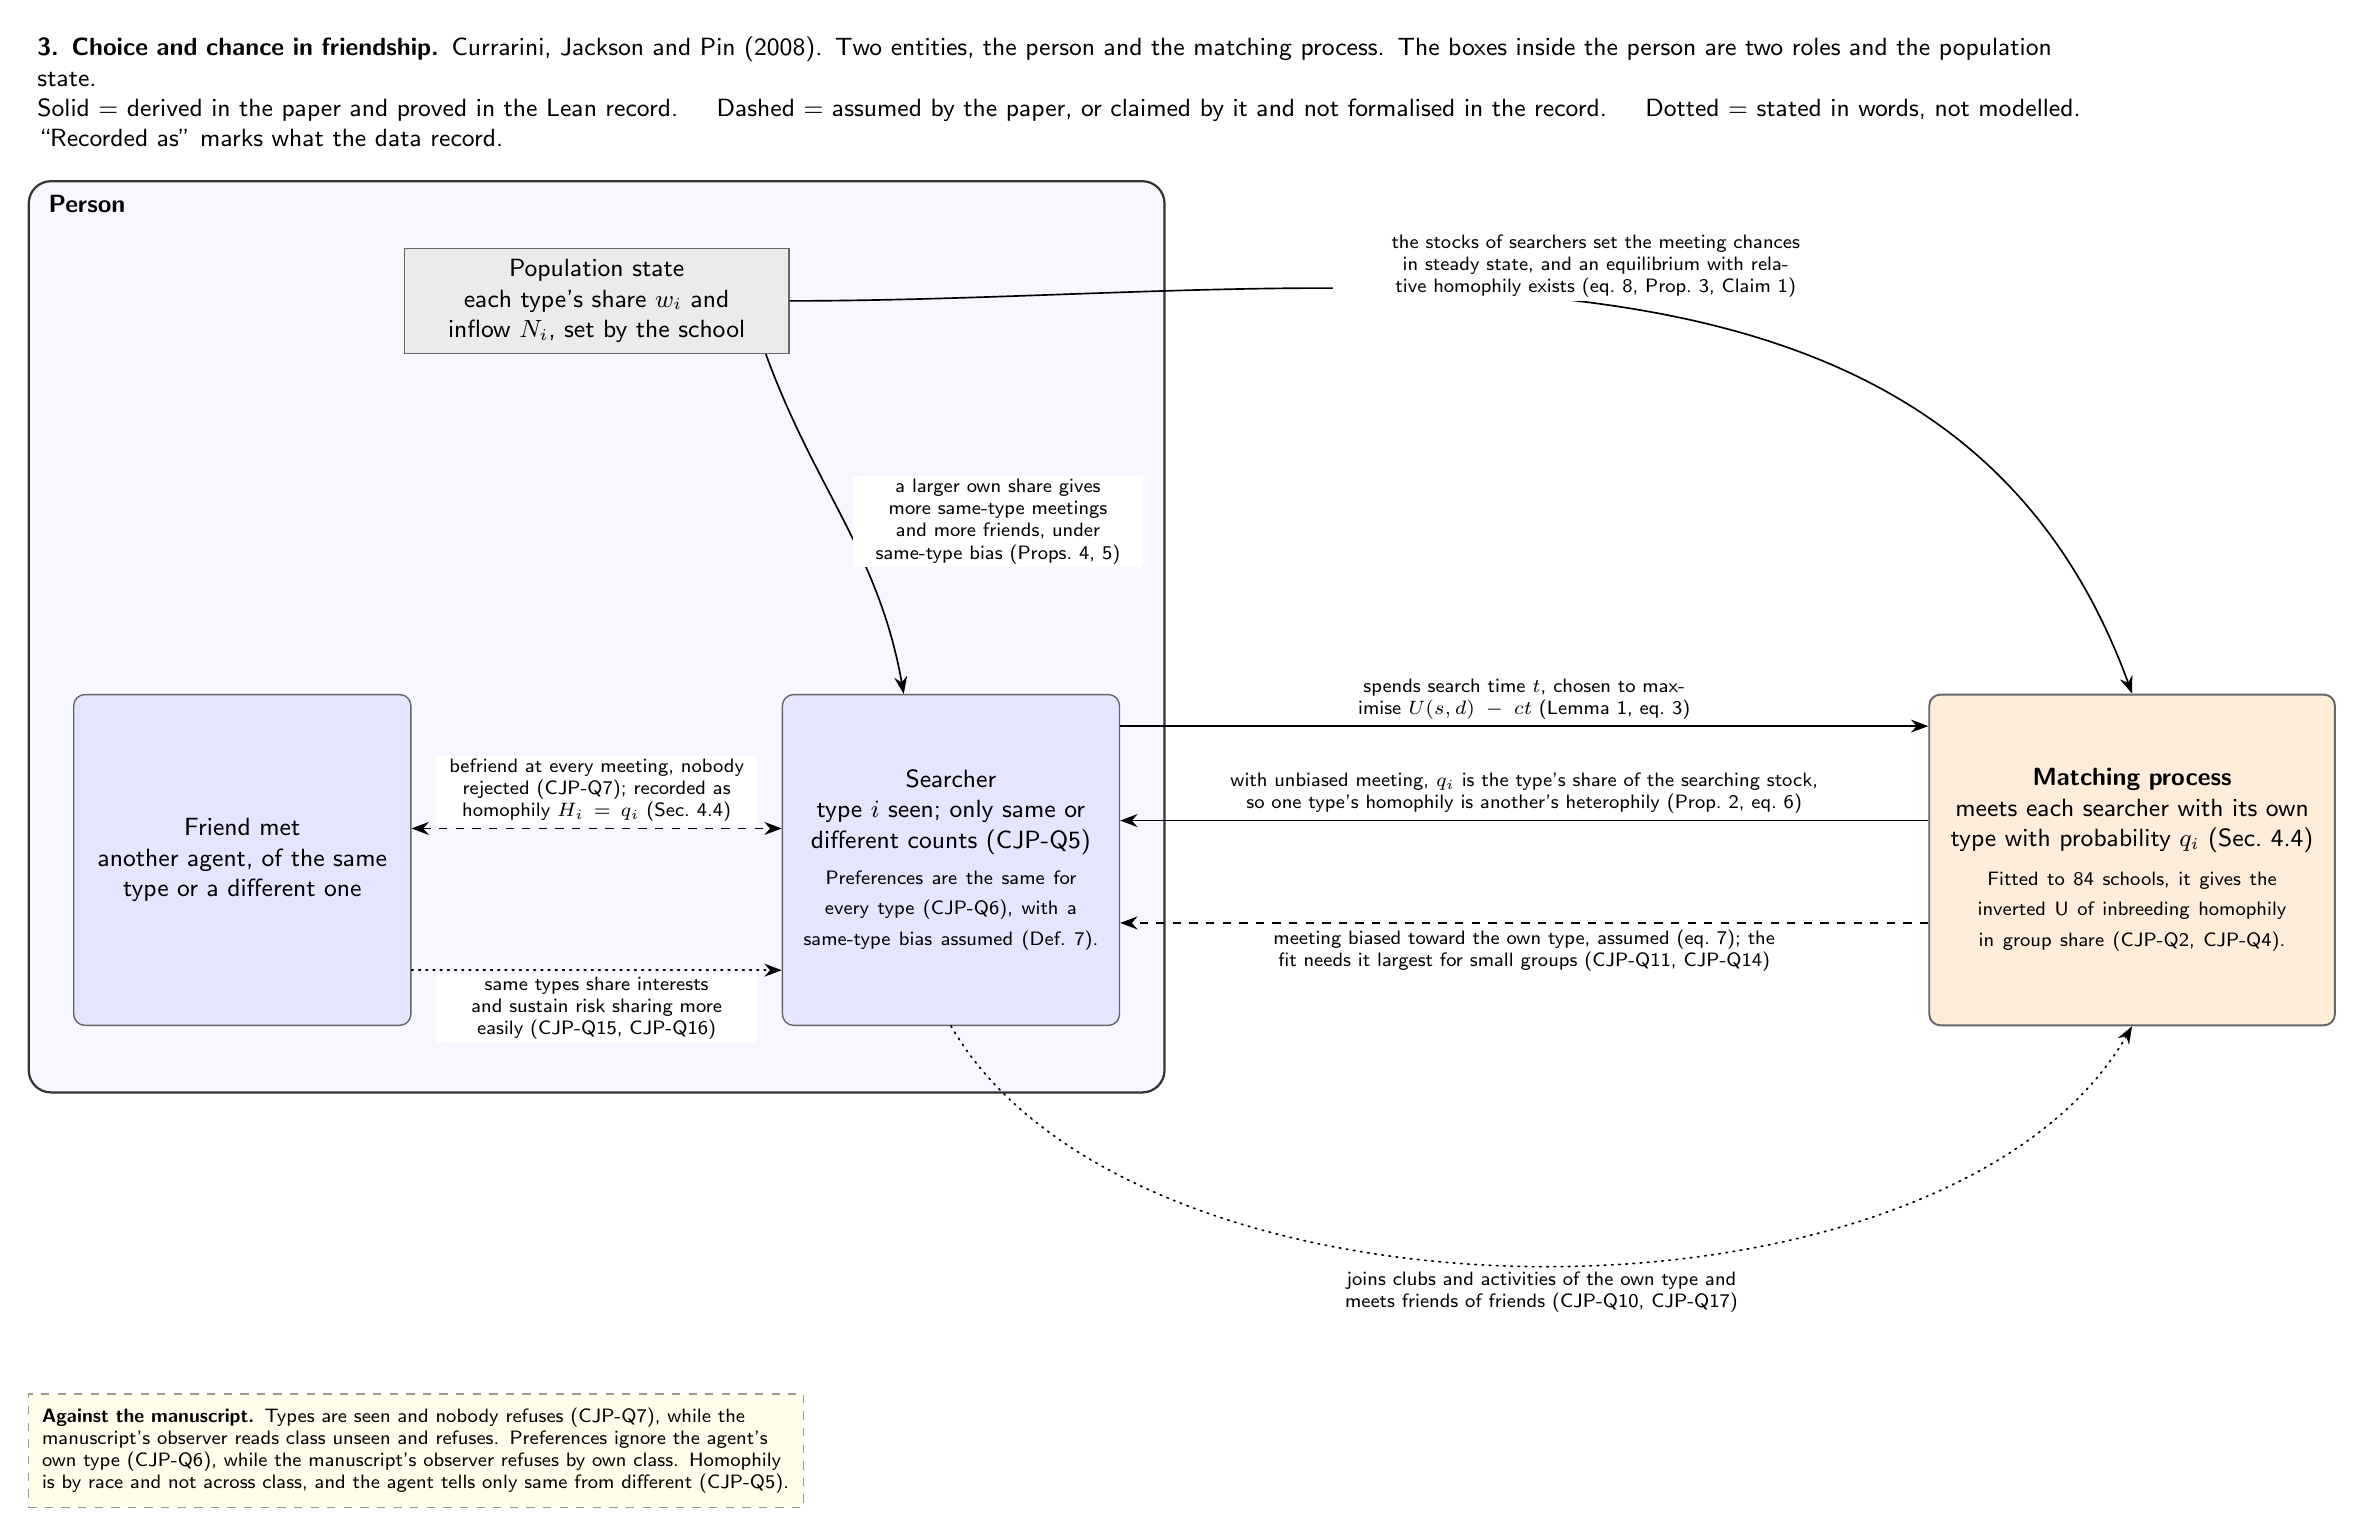
\begin{tikzpicture}
\node[pop]  (Pop) at (4.5,8.6) {Population state\\ each type's share $w_i$ and inflow $N_i$, set by the school};
\node[role] (FM)  at (0,1.5)   {Friend met\\ another agent, of the same type or a different one};
\node[role] (S)   at (9,1.5)   {Searcher\\ type $i$ seen; only same or different counts (CJP-Q5)\\[2pt] \scriptsize Preferences are the same for every type (CJP-Q6), with a same-type bias assumed (Def.~7).};
\begin{scope}[on background layer]
\node[entity, fit=(Pop)(FM)(S), inner xsep=16pt, inner ysep=24pt] (PBox) {};
\end{scope}
\node[etitle] at ([xshift=4pt, yshift=-2pt]PBox.north west) {Person};

\node[other] (M) at (24,1.5) {\textbf{Matching process}\\ meets each searcher with its own type with probability $q_i$ (Sec.~4.4)\\[3pt] \scriptsize Fitted to 84 schools, it gives the inverted U of inbreeding homophily in group share (CJP-Q2, CJP-Q4).};

\draw[jointgiven] ([yshift=4mm]FM.east) -- node[lab, pos=0.5, above=1pt, text width=4.0cm] {befriend at every meeting, nobody rejected (CJP-Q7); recorded as homophily $H_i=q_i$ (Sec.~4.4)} ([yshift=4mm]S.west);
\draw[open]    ([yshift=-14mm]FM.east) -- node[lab, pos=0.5, below=1pt, text width=4.0cm] {same types share interests and sustain risk sharing more easily (CJP-Q15, CJP-Q16)} ([yshift=-14mm]S.west);

\draw[settled] ([yshift=17mm]S.east) -- node[lab, pos=0.5, above=1pt, text width=6.6cm] {spends search time $t$, chosen to maximise $U(s,d)-ct$ (Lemma~1, eq.~3)} ([yshift=17mm]M.west);
\draw[settled] ([yshift=5mm]M.west) -- node[lab, pos=0.5, above=1pt, text width=7.6cm] {with unbiased meeting, $q_i$ is the type's share of the searching stock, so one type's homophily is another's heterophily (Prop.~2, eq.~6)} ([yshift=5mm]S.east);
\draw[given]   ([yshift=-8mm]M.west) -- node[lab, pos=0.5, below=1pt, text width=7.6cm] {meeting biased toward the own type, assumed (eq.~7); the fit needs it largest for small groups (CJP-Q11, CJP-Q14)} ([yshift=-8mm]S.east);
\draw[open]    (S.south) to[out=-60, in=-120, looseness=0.8] node[lab, pos=0.5, below=1pt, text width=6.2cm] {joins clubs and activities of the own type and meets friends of friends (CJP-Q10, CJP-Q17)} (M.south);
\draw[settled] (Pop.east) to[out=0, in=110] node[lab, pos=0.5, above=1pt, text width=6.6cm] {the stocks of searchers set the meeting chances in steady state, and an equilibrium with relative homophily exists (eq.~8, Prop.~3, Claim~1)} (M.north);
\draw[settled] ([xshift=-3mm]Pop.south east) to[out=-70, in=100] node[lab, pos=0.5, anchor=west, xshift=3pt, text width=3.6cm] {a larger own share gives more same-type meetings and more friends, under same-type bias (Props.~4, 5)} ([xshift=-6mm]S.north);

\node[note, anchor=north west] at ([yshift=-6mm]current bounding box.south west) {\textbf{Against the manuscript.} Types are seen and nobody refuses (CJP-Q7), while the manuscript's observer reads class unseen and refuses. Preferences ignore the agent's own type (CJP-Q6), while the manuscript's observer refuses by own class. Homophily is by race and not across class, and the agent tells only same from different (CJP-Q5).};
\node[head] at ([yshift=8pt]current bounding box.north west) {\textbf{3. Choice and chance in friendship.} Currarini, Jackson and Pin (2008). Two entities, the person and the matching process. The boxes inside the person are two roles and the population state.\\ \legend};
\end{tikzpicture}

\end{document}
